\chapter{Background}
\section{Existing alternatives}
As of writing this paper, only very few tools support monitoring of STP topologies.
The ones we found are LoriotPro\cite{LoriotPro}, LiveAction\cite{LiveAction} and L2Discover\cite{L2Discover}.
Only the source code for L2Discover is openly available, the other two are proprietary software.
The company SolarWinds has an open vote on their website on whether or not to include this feature in the future since 2014\cite{thwackSW}.
LoriotPro and L2Discover use the SNMP for their topology discovery.
STP is only used to discover unused and duplicate links.
The Generator described in this paper uses only STP, thus not needing SNMP capable devices.

\section{Technologies used}
\subsection{STP}
\subsubsection{STP Packets}
\begin{figure}[h]
    \centering
    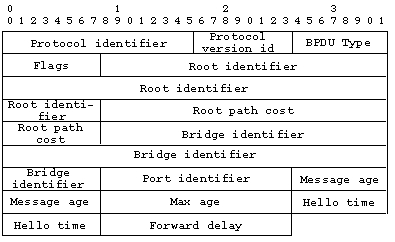
\includegraphics[width=0.8\textwidth]{stp_bpdu.png}
    \caption{An STP BPDU}
    \label{fig:stp_bpdu}
\end{figure}
In this section we will explain the parts of an STP Bridge Protocol Data Unit (BPDU), as seen in Figure~\ref{fig:stp_bpdu}, used in this project.
\begin{itemize}
    \item \textbf{Flags}: The Flags Byte is used for the \textit{Topology Change} and \textit{Topology Change Acknowledgement} flags.
    \item \textbf{Root/Bridge Identifier}: The Identifier conists of three parts and has the same layout for the Root and regular bridges:
        \begin{itemize}
            \item Priority (4 Bits): A value between 0 and 61440 configurable in increments of 4096
            \item System ID Extension (12 Bits): Used for keeping the Bridge ID unique if multiple VLANs are configured for a Bridge
            \item Bridge MAC (6 Byte): The MAC address of the Bridge
        \end{itemize}
        The Identifier is used to determine the Root of the tree, as well as port statuses between Bridges sharing the same distance from the Root.
    \item \textbf{Root Path Cost}: The Root Path Cost is the sum of all Port Costs (which can be configured in the Bridge) along the current path. The Root Path Cost in packets sent by the Root is 0.
    \item \textbf{Message Age}: The Message Age is the number of Bridges that have been passed (in addition to the Root) along the current path.
\end{itemize}
\subsubsection{Building the Tree} 
How does STP work?
\subsection{PCAP}
PCAP 
\subsection{JSON}
JSON very brief
